\documentclass[slidestop,compress,red,mathserif]{beamer}

\usepackage{pgf,pgfarrows,pgfnodes,pgfautomata,pgfheaps,pgfshade}
\usepackage{amsmath,amssymb}
\usepackage{comment}
\usepackage{graphicx}
\usepackage[english]{babel}
\usepackage{tabularx}
\usepackage{xcolor}
\usepackage{multirow}
\usepackage{marvosym}
\usepackage{natbib}
\usepackage{ulem}
\usepackage{wasysym}

\setbeamersize{text margin left=6mm, text margin right=2mm}

\mode<presentation>
{
%\usetheme{Warsaw}
%\usetheme{Rochester}
%\usetheme{Madrid}
%\usetheme{Pittsburgh}
%\usetheme{Antibes}
%\usetheme{Montpellier}
%\usetheme{Berkeley}
%\usetheme{PaloAlto}
%\usetheme{Goettingen}
%\usetheme{Marburg}
%\usetheme{Hannover}
%\usetheme{Berlin}
\usetheme{Ilmenau}
%\usetheme{Dresden}
%\usetheme{Darmstadt}
%\usetheme{Frankfurt}
%\usetheme{Singapore}
%\usetheme{Szeged}
%\usetheme{Copenhagen}
%\usetheme{Malmoe}
\setbeamercovered{transparent}
}

% Choose color scheme
%
\usecolortheme{default}
%\usecolortheme{sidebartab}
%\usecolortheme{albatross}
%\usecolortheme{beetle}
%\usecolortheme{crane}
%\usecolortheme{dove}
%\usecolortheme{fly}
%\usecolortheme{seagull}
%\usecolortheme{lily}
%\usecolortheme{orchid}

\beamertemplateballitem
%\setbeamertemplate{footline}{\insertframenumber/\inserttotalframenumber}

\defbeamertemplate*{footline}{shadow theme}
{%
  \leavevmode%
  \hbox{\begin{beamercolorbox}[wd=2.\paperwidth,ht=2.5ex,dp=1.125ex,leftskip=.3cm plus1fil,rightskip=.3cm]{author in head/foot}%
    \usebeamerfont{author in head/foot}\insertframenumber\,/\,\inserttotalframenumber\hfill%\insertshortauthor
  \end{beamercolorbox}%
  \begin{beamercolorbox}[wd=.5\paperwidth,ht=2.5ex,dp=1.125ex,leftskip=.3cm,rightskip=.3cm plus1fil]{title in head/foot}%
    \usebeamerfont{title in head/foot}%\insertshorttitle%
  \end{beamercolorbox}}%
  \vskip0pt%
}

% number sets
\def\N{\hbox{I \kern-.5em N}}
\def\R{\hbox{I \kern-.5em R}}
\def\Q{\hbox{\hspace*{.25em}{\sf I} \kern-.83em Q}}
\def\T{\rm T}  %%%%  \rm pour roman (ecriture normale)
\def\Z{\rm Z}
\def\ZZ{\hbox{\sf  Z \kern-.8em Z}}
\def \Zplus        {\ZZ^{+}}
\def \bigm {\textsc{penal}}
\def \dst {\textsc{dst}}
\def \src {\textsc{src}}
\def \zlp {z^{\star}_{\textsc{lp}}}
\def \zilp {{\tilde z}_{\textsc{ilp}}}
\def \l    {\textnormal{\textsc{l}}}
\def \Gp   {G_{\textsc{p}}}
\def \Gl   {G_{\l}}
\def \Vp   {V_{\textsc{p}}}
\def \Vl   {V_{\l}}
\def \Ep   {E_{\textsc{p}}}
\def \El   {E_{\l}}
\def \cost {\textsc{cost}}
\def \srlg {\textsc{srlg}}

% number sets
\def \best {\textsc{best}}
\def  \N            {\hbox{I \kern-.5em N}}
\def \RR {\mathbb{R}}
\def \Rplus {\RR^+}
\def  \Z            {\rm Z}
\def  \Zplus        {\Z^+}
\def  \Zplusn       {\Zplus_n}
\def  \ZZ           {\hbox{\sf  Z \kern-.8em Z}}
\def \Z {\mathbb{Z}}

\logo{%
    
\includegraphics[width=2.cm,keepaspectratio]{Figures/ConULogo_CMYK.eps}~%
}

\title[My Title]{Accident prediction in time and space}
\author[My~Name]{
\textbf{Timothée Guédon, Antoine Hébert}}
\institute[My Institute/company]
{Concordia University \\ Computer Science and Software Engineering Department}
\date[]{April 15, 2019}

\begin{document}

\begin{frame} % Cover slide
\titlepage
\end{frame}

% layout of the presentation
\AtBeginSubsection[]
{
  \begin{frame}<beamer>
    \frametitle{Layout}
    \tableofcontents[currentsection,currentsubsection]
  \end{frame}
}

\begin{frame}
\frametitle{Table of Contents}
\tableofcontents
\end{frame}

\AtBeginSection[]
{
  \begin{frame}
    \frametitle{Table of Contents}
    \tableofcontents[currentsection]
  \end{frame}
}

%-------------------------------------------------
\section{Introduction}
%-------------------------------------------------

% -------------------------------------------------------------------------------------------------------------------

\begin{frame}
\frametitle{Road accident prediction}

\begin{scriptsize}

\begin{itemize}
\item[] \textbf{Context}:
  \begin{itemize}
    \item Road accidents implies millions of people deaths and injuries every year.
		\item Human and economic impact on society.
    \item Master’s thesis of Antoine Hébert in a different context.
  \end{itemize}

\item[] \textbf{Our goals}:
  \begin{itemize}
    \item Dataset analysis.
  	\item Finding key insights in accident prediction.
  	\item Identifying issues related to class imbalance and geo-spatial data.
  \end{itemize}
\end{itemize}

\end{scriptsize}

\end{frame}

% -------------------------------------------------------------------------------------------------------------------

\begin{frame}
\frametitle{Datasets}

\begin{footnotesize}
We used open datasets from Open Canada.

\begin{itemize}
\item[] \textbf{National Collision Database (NCDB)}:
  \begin{itemize}
  	\item All vehicle collisions reported by the police from 2012 to 2017 in Montreal.
  	\item Date and time, severity, number of death and injury, number of vehicles, localization, speed limit etc.
  \end{itemize}
\item[] \textbf{National Road Network}:
  \begin{itemize}
    \item Shape of the road, how roads are
connected together, the mail addresses on the street, the number of lanes in each direction and the
type of pavement.
  \end{itemize}
\item[] \textbf{Climate data - Hourly Data Report}:
  \begin{itemize}
    \item For each position and hour, the dataset provides the temperature, the humidity, the wind speed and direction, the visibility, the atmospheric pressure etc.
  \end{itemize}
\end{itemize}

\end{footnotesize}

\end{frame}

% -------------------------------------------------------------------------------------------------------------------


\begin{frame}
\frametitle{Tree-based algorithms}
We chose to focus on tree-based algorithms because it has proven its efficiency on accident prediction.
\begin{itemize}
\item[] \textbf{Related work on accident prediction}:
  \begin{itemize}
    \item Extensive use of decision trees in several form. (Athanasios Theofilatos, A. 2017, Joaquín Abellán, 2013, Lei Lin 2014, Li-Yen Chang 2005)
    \item Recently, deep learning algorithms (LSTM and CNN architectures for example) (Zhuoning Yuan, 2018, Quanjun Chen 2016)
  \end{itemize}
\item[] \textbf{Chosen algorithms}:
  \begin{itemize}
  	\item Random Forest
    \item Balanced Random Forest
    \item Gradient Boosted Trees (GBT) - XGBoost implementation
  \end{itemize}
\end{itemize}
\end{frame}


%-------------------------------------------------
\section{Methods}
%-------------------------------------------------

\begin{frame}
	\frametitle{Generating the negative samples}
	\begin{itemize}
    \item Every time an accident did not happen is considered a negative sample.
		\item A sample from the cartesian product between all dates (between 01/01/2012 and 31/12/2017) and all roads.
		\item Generation of 5 million negative samples for about 200 000 positive samples.
	\end{itemize}
\end{frame}

\begin{frame}
	\frametitle{Some feature engineering}
	\begin{itemize}
		\item Computing the distances between GPS coordinates (taking into account earth curvature)
		\item Making the dates and times cyclic
		\item Creating missing points on the roads
    \item Interpolating weather statistics by averaging data from several stations
    \item etc...
	\end{itemize}
\end{frame}

\begin{frame}
	\frametitle{Area under PR curve}
	\begin{itemize}
    \item ROC Curve : false positive rate VS true positive rate
    \begin{equation*}
			FPR = \frac{FP}{FP+TN},  TPR = \frac{TP}{TP+FN}
		\end{equation*}
		\item PR Curve : true positive rate VS precision
    \begin{equation*}
			TPR = \frac{TP}{TP+FN},  Precision = \frac{TP}{TP+FP}
		\end{equation*}
    \item Data imbalance imply decrease of TP and increase of FN
    \item Therefore, area under PR exhibits larger difference than are under ROC
	\end{itemize}
\end{frame}


%-------------------------------------------------
\section{Balanced Random Forests}
%-------------------------------------------------

\begin{frame}
\frametitle{Remainder: Random Forests}
\begin{itemize}
  \item[] \textbf{Remainder}
    \begin{itemize}
    	\item Random Forests (\cite{Breiman2001}) are combinations of fully-grown decision trees.
    	\item Each tree is trained on a random sample of the data and a random sample of the features.
    \end{itemize}

  \item[] \textbf{Weighted Random Forests (WRF)}:
    \begin{itemize}
      \item A solution to imbalance.
      \item Add weights to the classes when growing the tree (in the Gini coefficient).
      \item Add weights to the classes at the voting time.
    \end{itemize}

\end{itemize}
~~~~~~~~~~~~~~~
\end{frame}


\begin{frame}
\frametitle{Solution to imbalance}
\begin{itemize}
  \item[] \textbf{Balanced Random Forests (BRF)}:
    \begin{itemize}
      \item Another solution to imbalance.
      \item Combine undersampling and ensemble method versus loss of information.
      \item For each tree : Randomly draw sample of same size from majority (with replacement) and minority class.
      \item The rest of the algorithm is identical to Random Forests
    \end{itemize}

  \item[] \textbf{BRF versus WRF}:
    \begin{itemize}
      \item No clear winner ! But...
      \item WRF - More vulnerable to noise on minority class
      \item BRF - More computationally efficient because use less data (subsampling)
      \item BRF - Easier to implement
    \end{itemize}

\end{itemize}
\end{frame}


\begin{frame}
\frametitle{Implementation of BRF in Spark}
\begin{itemize}
  \item[] \textbf{Existing implementation of RF in Spark}
    \begin{itemize}
    	\item To manage the subsampling of the dataset, Spark's scala implementation use the Poisson distribution.
      \item The Poisson distribution is used to compute the probability of an event to occur at a given time.
    	\item To know how many times a given sample will be in the subsample of a given tree (can be 0 times), we use "distribution sampling" of 1 element.
      \item (Distribution sampling: Get a random sample following a given distribution)
    \end{itemize}
  \item[] \textbf{Our modifications}:
    \begin{itemize}
      \item Instead of creating one Poisson distribution (with the "p" parameter and a seed) we create two Poisson distributions:
    	\item[]
      \begin{itemize}
      	\item One for the distribution of the "positive" samples,
        \item Another for the distribution of the "negative" samples.
      \end{itemize}
    \end{itemize}
\end{itemize}
\end{frame}

\begin{frame}
\frametitle{Experimenting with our BRF implementation}
\begin{itemize}
  \item Area Under PR : 99,3\% for WRF VS 99,7\% for BRF
  \item F1 score : 99\% for WRF VS 98\% for BRF (which proves that F1 score can be misleading)

\end{itemize}

\centering
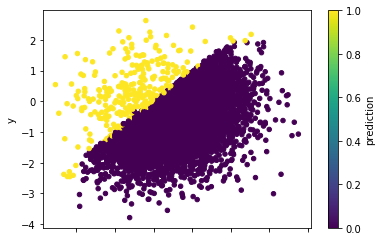
\includegraphics[height=3.5cm, keepaspectratio]{Figures/BRF.png}
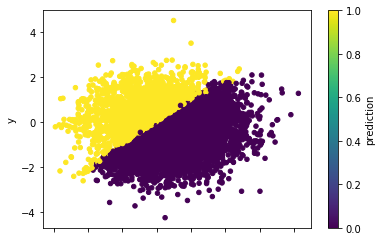
\includegraphics[height=3.5cm, keepaspectratio]{Figures/WRF.png}

\end{frame}

%-------------------------------------------------
\section{Big Data related issues}
%-------------------------------------------------

\begin{frame}
	\frametitle{Dataset generation}
	\begin{itemize}
		\item Using slurm-based (scheduler) cluster to increase the dataset generation's speed.
    \item Tricks to increase the generation speed and reduce the memory consumption.
	\end{itemize}
\centering
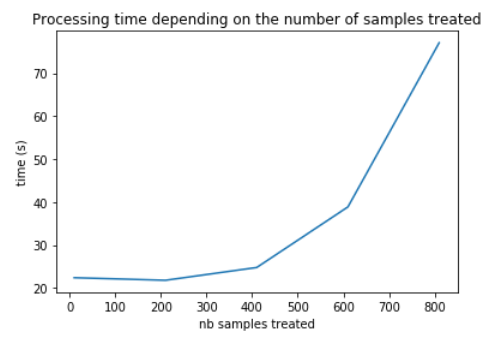
\includegraphics[height=3.5cm, keepaspectratio]{Figures/timeVSsamples_generatepositivesamples.png}
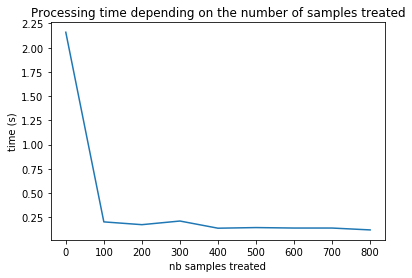
\includegraphics[height=3.5cm, keepaspectratio]{Figures/timeVSsamples_generatepositivesamples_after.png}
\end{frame}

\begin{frame}
	\frametitle{Spark VS Dask}
	\begin{itemize}
    \item[] \textbf{Advantages of using Dask over Spark}
      \begin{itemize}
      	\item Mimic the pandas dataframe API
        \item Lighter than Spark
      	\item Designed to be more flexible in terms of applications and algorithms
      \end{itemize}
    \item[] \textbf{Why we switched for Spark}
      \begin{itemize}
        \item We found ourselves writing a lot more code using Dask than using Spark
        \item We found Spark easier to use for processing the dataset in batch
        \item Spark's map-reduce and shuffling operations are very handy
        \item Spark ML pipelines allow to create pipelines of preprocessing easily
      \end{itemize}
	\end{itemize}
\end{frame}

%-------------------------------------------------
\section{Results}
%-------------------------------------------------

\begin{frame}
	\frametitle{Comparison between the algorithms}
	\begin{itemize}
		\item Random forest
		\item Balanced random forest
		\item XGBoost
	\end{itemize}
\end{frame}

\begin{frame}
	\frametitle{Key features identified}
	\begin{itemize}
		\item The most important features seem to be the time and location of the vehicle, followed by some road's features like the type of road (highway for example) and the street length.
    \item Finally, comes wome weather features like the visibility, the wind and the humidity.
	\end{itemize}
\centering
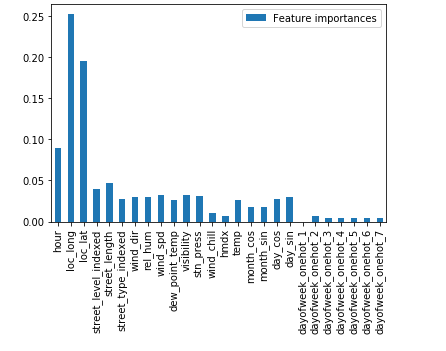
\includegraphics[height=4cm, keepaspectratio]{Figures/features.png}
\end{frame}

%-------------------------------------------------
\section{Conclusion}
%-------------------------------------------------

\begin{frame}
	\frametitle{Conclusion}
	\begin{itemize}
    \item We found some key features that can explain the occurence of accidents.
    \item We identified some issues related to class imbalance and big data analytics.
    \item Future work would include tuning the XGBoost classifier, testing lightGBM classifier, assing some datasets like a road works dataset.
    \item The code can be found on Github at https://github.com/GTimothee/accident-prediction-montreal
	\end{itemize}
\end{frame}

% -------------------------------------------------------------------------------------------------------------------------
% -------------------------------------------------------------------------------------------------------------------------
%% -------------------------------------------------------------------------------------------------------------------------

\begin{frame}[allowframebreaks]
\frametitle{References}

{\scriptsize

\bibliographystyle{plainnat}
\bibliography{Biblio}

}


\end{frame}

\end{document}
